%!TEX root = ../thesis.tex
%*******************************************************************************
%****************************** Second Chapter *********************************
%*******************************************************************************

\chapter{Deep Learning}

\ifpdf
     \graphicspath{{Figs/Chapter2/}}
\else
    \graphicspath{{Chapter2/Figs/Vector/}{Chapter2/Figs/}}
\fi

There are many tasks which are hard to write algorithms for. For example, writing an algorithm the identifies a type of fruit using a picture of the fruit is a challenging undertaking. You could try to solve this problem by asking a number of yes or no questions which help whittle down the possibilities to a handful of fruit. A sensible question to ask might be - "Is the fruit round?". If the answer was yes, we could immediately discard options like strawberries, pineapples and pears. Another sensible question to ask might be - "Is the fruit orange?". If the answer is yes, again we could immediately discard unlikely candidates. Finally we could ask - "Is the fruit rough?". And if the answer was no, we could be pretty sure the picture we were looking at was an orange. \newline
The problem with this approach is that it is very brittle. You could ask a question that would lead a high likelihood that the image was indeed an orange, however the image may not in fact be an orange. For example apples could also be round, orange and smooth. More questions could try to disambiguate the two types of fruit, but there is enough variation in fruit that our algorithm could be confused. Writing rules in this way also is not scalable. There are a large number of types of fruits, and writing questions to determine each one quickly becomes intractable, let alone questions that help distinguish similar fruit. \newline 
Machine learning (ML) is used to solve such tasks, as well as others such as weather prediction, stock price forecasting and risk modelling ~\citep{hastie2009elements}. ML is the process of using data to build prediction models where these models typically output discrete (classification) or continuous (regression) values. ML uses a number of learning paradigms ~\citep{murphy2012machine}, including supervised learning, unsupervised learning and reinforcement learning, to train models. The models can be divided into three classes, namely shallow, deep and probabilistic ~\citep{hastie2009elements, murphy2012machine}. The models are trained using data to accomplish a task. \newline
\newpage
This chapter presents a discussion on the supervised learning paradigm, an analysis of the convolutional network ~\citep{lecun1998gradient} and recurrent network ~\citep{werbos1988generalization} deep learning models, and a discussion on deep learning training techniques, including dropout ~\citep{srivastava2014dropout} and batch normalisation ~\citep{ioffe2015batch} regularisation. 


%********************************** %First Section  **************************************

\section{Supervised Learning}

ML prediction models take as input a set of features. These features are attributes of a data sample. For example in the fruit prediction task mentioned above, input features would be the attributes of a fruit. They would include characteristics such as shape, colour, texture and size. These inputs are provided to a model that maps to outputs. In the example above, these outputs would be types of fruit, and could represent values such as oranges, apples, strawberries and pineapples, amongst others. The model is then taught (trained) to identify the correct fruit (output) based on the features (input) it receives. This type of training paradigm is called supervised learning \citep{bishop2006pattern, hastie2009elements, murphy2012machine}. \newline

\begin{figure}[H]
  	\caption{Supervised Learning}
   	\centering
    	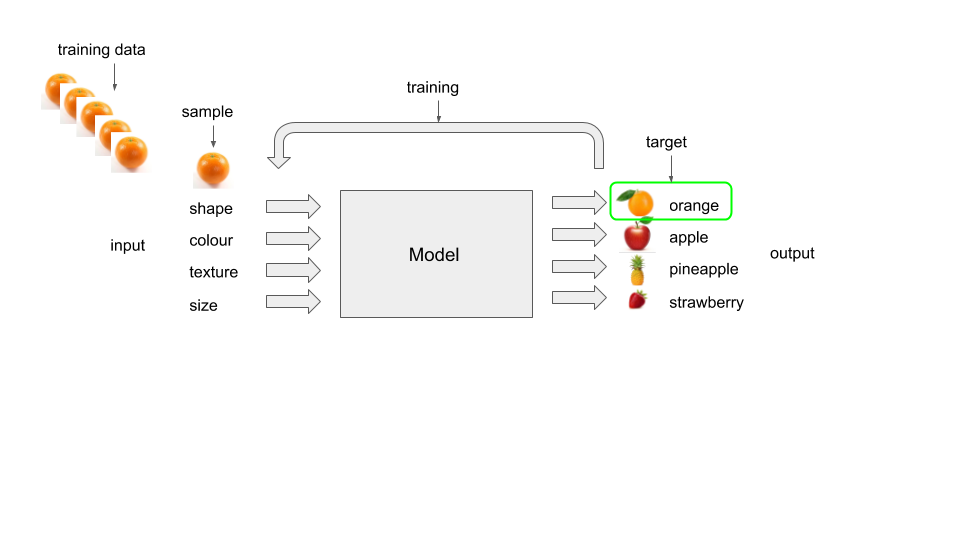
\includegraphics[width=\textwidth]{supervised_learning}
\end{figure}

Features can be continuous valued or discrete, where discrete values are referred to as categorical variables. Outputs can also be continuous or discrete, where discrete outputs are known as classes. Input-output pairs comprise a dataset which is represented as follows, \begin{math} D = \{(x_i, y_i)\}_{i=1}^N \end{math}, where \begin{math} D \end{math} is the dataset, \begin{math} x_i \end{math} is the input sample and \begin{math} y_i \end{math} is the output label. The model has to learn the correct mapping of input to output - features to label. We use data samples to train the model to recognise which features are correlated with which labels. The model is trained using an algorithm where it is shown a sample and it outputs what it believes is the correct label. If it gets the label wrong, an objective function is used to assess how large the error was, and the model is adjusted. We try to minimise this error during training, and because we try to minimise the objective function value, it is called a loss function. The algorithm is expressed as follows: \bigbreak

\begin{algorithm}[H]
	\SetAlgoLined
	\textbf{Input} 
	Training set \begin{math} D = \{(x_i, y_i)\}_{i=1}^N \end{math}, samples and labels\;
  	\begin{math} S_{batch} \gets sample(S, b) \end{math} // sample a minibatch of size \begin{math} b \end{math} \\
	 \For{(x, y) \begin{math} \in S_{batch} \end{math}}{
     		\begin{math} y \gets predict(x, y) \end{math} // predict label for sample \\
		\begin{math} e \gets y' - y \end{math} // compute error
     		}
	Update model w.r.t. \begin{math}  e \end{math}
	\caption{Supervised Learning}
\end{algorithm} \bigbreak

The model tries to build an approximation of the underlying distribution of data. Two important assumptions are made about the data, that the samples are independent and therefore order invariant, and that the data is identically distributed - that it is generated by the same underlying process for all samples. This type of data is called independently and identically distributed (IID) data. In the above example, the model will attempt to build decision boundaries around fruit classes given the features of the fruit. We can visualise this process in a 2-Dimensional setting using two fruit features, shape and colour. We generate a synthetic dataset using random number generation and then assign classes to our randomly generated classes, see Figure 4 below.

\begin{figure}[H]
  	\caption{Model Decision Boundary}
   	\centering
    	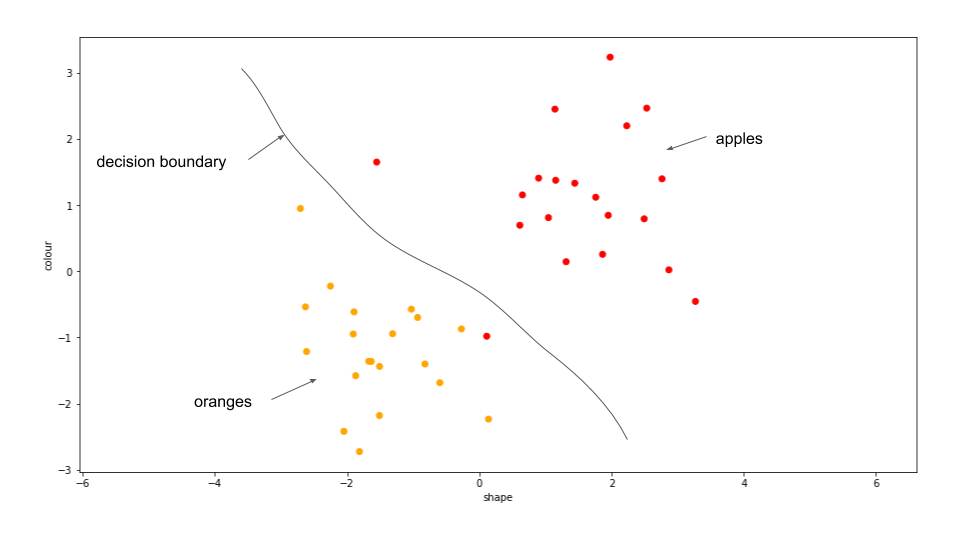
\includegraphics[width=0.8\textwidth]{oranges_and_apples_decision_boundary}
\end{figure}

Another class of data called non-IID data, where data samples are dependent and the sequence matters. These data are typically divided into training, validation and test sets for model training, where the type of data directly determines the best choice of model for mapping input to output. The choice of model also affects how the surface will look. A popular method of optimisation is gradient decent. Model updates are computed based on the first order parameter partial derivatives of the loss function.If the model only had three parameters, we could once again visualise how a possible loss surface might look. The job of the training algorithm, is to guide our model parameters toward a global minimum, in practice a local minimum is the best we can achieve.


%********************************** %Second Section  **************************************

\section{Deep Learning Models}

Deep learning models have become the preferred models for classification and regression tasks, and more broadly machine learning tasks. The reason for this is that deep models solve a major problem with shallow models - selecting the best features with which to represent samples ~\citep{Goodfellow-et-al-2016}. The problem of feature selection had resulted in a number of a methodology used during shallow model development: feature engineering. Feature engineering includes techniques such as bucketing, crossing, hashing and embedding ~\citep{murphy2012machine, Goodfellow-et-al-2016}. These techniques are designed to build sample representation that will result in high classification and regression accuracy. Deep models discovery optimal representations automatically, hence their superior performance on a number of machine learning tasks. \newline
Multilayer perceptrons (MLP) were the early deep learning models implemented as feed-forward neural networks consisting of $N$ layers, applied to an input vector $ x $. These models compute un-normalised scores known as logits, for each of the possible $ M $ outputs, classes and values in classification and regression respectively. They do this by executing a number of steps in an algorithm called the forward pass. Each step is called a layer, where an MLP can consist of a number of layers. A basic MLP consists of three of these layers, an input, hidden and output layer. The MLP computes a linear combinations of input features, then transforms the representation using a nonlinear hidden activation layer, before computing a linear combination of outputs. MLP models can be defined as follows:

\begin{subequations}
\begin{gather}
	f_0 = x \\
	f_i=\sigma_i(W_if_{i - 1} + b_i) \quad i \in [1, N]
\end{gather}
\end{subequations}

where $f_0$ is the input layers, $f_i$ is the respective computation layer. Each layer has a particular number,  $m_i$, of neurons. The parameters of a layer consist of a matrix $W_i \in \mathbb{R}^{m_i \times m_{i-1}}$ and bias vector $b_i \in  \mathbb{R}^{m_i}$. Each layer also has a non-linear activation function $\sigma_i$. \newline
Loss functions are used to train deep models under a supervised learning paradigm. The error computed by the loss is used in a process called back propagation - the computing of parametric first order partial derivatives, and the adjustment of the parameters in direction and magnitude of their respective derivative. This process is given by:

\begin{subequations}
\begin{gather}
	\frac{\partial E} {\partial W_n} = \frac{\partial F} {\partial W}(W_n, X_{n-1})\frac{\partial E} {\partial X_n} \\
	\frac{\partial E} {\partial X_{n-1}} = \frac{\partial F} {\partial X}(W_n, X_{n-1})\frac{\partial E} {\partial X_n} 
\end{gather}
\end{subequations}

where $\frac{\partial F} {\partial W}(W_n, X_{n-1})$ is the Jacobian of $F$ with respect to $W$ evaluated at the point $(W_n, X_{n-1})$, and  $\frac{\partial F} {\partial X}(W_n, X_{n-1})$ is the Jacobian of $F$ with respect to $X$. The Jacobian of a vector function is a matrix containing the partial derivatives of all the outputs with respect to all the inputs. Together the forward pass algorithm and back propagation, allow the automatic discovery of the most meaningful representation to compute the model output. We refer the reader to ~\citep{Goodfellow-et-al-2016} for a review on loss functions, as well as a more detailed discussion on the forward pass and back propagation. 

%********************************** %Convolutional Networks  **************************************

\subsection{Convolutional Networks}

MLPs suffer from an explosion of parameters  ~\citep{krizhevsky2012imagenet}. In fact when modelling a sample using a regular feed-forward network, we find that the number of model parameters grows exponentially. For example, a feed-forward network with $2$ hidden layers consisting of $512$ and $256$ neurons respectively, an output size of $10$ and an input sample shape of $\left [ \begin{matrix} 200 & 1 \end{matrix} \right] $, then the model ends up having: 


\begin{multline}
		total parameters = (X_D \times L_{D_i} + L_{D_i}) + (L_{D_i} \times L_{D_{i+1}} + L_{D_{i+1}}) \\ 
		+ \dots + (L_{D_{i+N-1}} \times L_{D_{N}} + L_{D_{N}}) \quad i \in [1, N]
\end{multline}

where $X_D$ is the input dimension size, $L_D$ is the number of nodes and $i$ is the layer number, for a total of $236,810$ parameters. Compounding this issue, is the incapability of MLPs to take advantage of structure in data, thus having no way of compensating for distributions of representations of the same conceptual sample. In order to cater for sample representation distribution variance, MLPs have to be larger, so as to have enough learning capacity to be able to hold sufficiently representative feature mappings ~\citep{lecun1998gradient}. \newline
Convolutional neural networks (CNN) have been developed to overcome both the above mentioned problems experienced by MLPs. CNNs make use of the convolutional operation during representation learning. This operation allows CNNs to achieve representation translation and location invariance ~\citep{simonyan2014very}. Translation invariance allows the CNN to build an object representation that is consistent under transformation, for example an image rotation would lead to a consistent final sample representation being generated. Locality invariance allows the model to generate the same representation a sample concept if the concept signal shifts along the dimensions of the representation. These properties allow CNNs to model the true distribution of samples using fewer parameters and smaller datasets. In the following we discuss the CNN forward pass algorithm. \newline
\textbf{Convolutional Layers.} CNNs perform a convolutional operation on a sample using a trainable representation filter. The operation constructs latent features of the sample by generating a feature map representation. Every filter is N-dimensional, for example 2-dimensional, and small spatially (along width and height), but extends through the full depth of an N-dimensional input volume. During the forward pass, each filter is convolved across the width and height of the input volume, where the element-wise dot product is computed between the entries of the filter and the input at any position. A 2-dimensional feature map is generated as a result, that gives the responses of that filter at every spatial position. Every convolutional layer has a set of corresponding filters, and each of them produce separate 2-dimensional feature maps, which are then stacked along the depth-dimension to produce an output volume. The size of the output volume is controlled by the hyperparameters of the convolutional layer: the filter size $F$ defines the width and height of the filters in the layer. Filters always have the same depth as the inputs to the layer. Depth $D$ of the layer defines the number of filters in the layer. Stride $S$ defines the number of entries by which we move the filter when convolving it along the input volume. Padding $P$ refers to the number of 0 entries we add to the input volume along the width and height dimensions. This parameter is useful in that it gives us more control over the desired size of the output volume and is used to ensure that the output volume has the same width and height as the input volume ~\citep{DLIndaba2017}.\newpage
The convolution forward pass is given by:

\begin{equation}
	O_{ij}^{d} = b_d + \sum_{a=0}^{F - 1}\sum_{b=0}^{F - 1}\sum_{c=0}^{I - 1}W_{a,b,c,d}X_{i+a,j+b,c}^{pad}
\end{equation}

where $O$ is the value of the output volume at position $(i,j,d)$, $b$ bias vector of shape $\left [ \begin{matrix} D \end{matrix} \right]$, $W$ is the weight tensor of shape $\left [ \begin{matrix} F & F & I & D \end{matrix} \right]$, $X$ is the padded input volume and $a, b, c$ are the volume dimensions. \newline
\textbf{Pooling Layers.} A pooling layer is used to reduce the spatial size of the representation. They are used to reduce the number of parameters in the network. Pooling layers provide latent features deeper int the network with a larger receptive field - input regions that they look at in order to represent larger sample surfaces. In particular, pooling stride gives deeper latent features much larger receptive fields so that they can effectively combine smaller features together. Pooling layers apply some 2-dimensional aggregation operation (usually a max, but others like average may also be used) to regions of the input volume. A pooling layer has no trainable parameters itself.  \newline
\textbf{Fully Connected Layers.} In order to compute the output of a CNN, a fully connected layer is required to flatten the output volume. This layer performs a tensor operation that computes an output vector $Y \in \mathbb{R}^{m}$. \newline
\textbf{Convolutional Backpropagation.} Computing parameter updates for convolutional filters is follows the same first order differential procedure used in backpropagation for MLPs. Assuming a loss function $L$ and having computed the derivative of this loss up to the output of the convolutional layer, $\frac{\partial L} {\partial O}$, in order to update the parameters the convolutional layer, we require the derivative of $L$ with respect to the weights and biases of the convolutional layer $\frac{\partial L} {\partial W}$ and $\frac{\partial L} {\partial b}$. We also require the derivative with respect to the inputs of the layer $\frac{\partial L} {\partial X}$ in order to propagate the error back to the preceding layers. \newline
The convolution backpropagation algorithm is thus given by:

\begin{subequations}
\begin{gather}
	\frac{\partial L} {\partial b} = \frac{\partial L} {\partial O}\frac{\partial O} {\partial b} \\
	\frac{\partial L} {\partial W_{a,b,c,d}} = \sum_{i=0}^{O_w - 1}\sum_{j=0}^{O_h - 1}\frac{\partial L} {\partial O_{ij}^{d}}X_{i+a,j+b,c}^{pad} \\
	\frac{\partial L} {\partial X_{m,n,c}^{pad}} = \sum_{i=0}^{O_w - 1}\sum_{j=0}^{O_h - 1}\sum_{d=0}^{D - 1}W_{m-i,n-j,c,d}\frac{\partial L} {\partial O_{ij}^{d}}
\end{gather}
\end{subequations}

%********************************** %Recurrent Networks **************************************

\subsection{Recurrent Networks}

Not all datasets are IID. Non-IID data presents itself in the form of sequences. Natural language is a good example of this, where sentences are comprised of a sequence of words. If we had to try to predict the next word from a set of sequence words, it may be useful to have memory of what came before. Feedforward networks like MLPs and CNNs do not have such a capability and can only map fixed-size input-data to their output labels. Recurrent Neural Networks (RNN) ~\citep{werbos1988generalization} solve this problem by generalising feedforward models to incorporate sequential dependencies. \bigskip

\textbf{Recurrent Layers.} RNNs build context by generating a representation of a window of data samples. This context is called the state vector, and is used to used in regression tasks such as time-series estimation, as well as classification tasks such as language model word classification to augment input sample representations. RNN layers are composed of cells ~\citep{DLIndaba2018}, in contrast to nodes in MLPs and CNNs. Cells are modular units that take as input a self-generated state (context), and output from previous cells. They generate a new state and output as they process a data sample. An RNN cell can thus be modelled as follows: 

\begin{equation}
	h_t = \sigma(W_{hh}h_{t-1} + W_{xh}x_t + b)
\end{equation}

where $h_t$ the cell output, and used as the state vector for input received as the next sequence entry. $\sigma$ is a nonlinear activation function, $W_{hh}$ are the state vector input parameters, $W_{xh}$ are the input parameters, $x_t$ is the input and $b$ is the bias. $h_t$ could then be used to predict the word for the next sequence entry, which would be given by:

\begin{equation}
	y_t = \sigma(W_{hy}h_{t} + b)
\end{equation}

\textbf{Backpropagation Through Time.} Back-propagation through time (BPTT) is a gradient-based process that computes parameter updates by chaining first order derivative cell outputs through sequence-time. An error signal is computed at the current sequence-time, and the first order derivative is computed against all sequence entries in a specific window, using the relative sequence-time-specific output. That time-specific error is then backprograted through the RNN layer to adjust the cell state and input parameters. A fixed sequence length is decided upfront for updating cell parameters. This is called truncated BPTT and has both training algorithm as well as compute resource advantages. \newpage
Assuming a loss function $L$, the gradient of the loss $E_t$ at time $t$ on $W_{hh}$ is a function of the current hidden state and model predictions $\hat{y_t}$ at time $t$:  

\begin{equation}
\frac{\partial E_t} {\partial W_{hh}} = \sum_{k=0}^{t}\frac{\partial E_t} {\partial \hat{y_t}}\frac{\partial \hat{y_t}} {\partial h_t}\frac{\partial h_t} {\partial h_k}\frac{\partial h_k} {\partial W_{hh}}
\end{equation}

One problem experienced by RNNs is the multiplicative effect of state vector derivates throughout sequence-time. This problem can be expressed as:

\begin{equation}
\frac{\partial h_t} {\partial h_k} = \prod_J\frac{\partial h_j} {\partial h_{j-1}}
\end{equation}

for $j$ from $k + 1$ to $t$. This multiplicative operation causes small gradients to become progressively smaller as the sequence window become larger, or become much larger. This is called the vanishing or exploding gradient problem and has lead to the development of RNN variant models such as Long Short-Term Memory ~\citep{hochreiter1997long} and Gated Recurrent Units ~\citep{cho2014learning}.


%********************************** %Third Section  **************************************

\section{Regularisation}

Model over parameterisation can lead to overfitting of in-sample data. This because the degrees of freedom available to estimate a function allow very complex nonlinear functions to be discovered, where these nonlinear functions are not representative of the generative process of the data. In fact, the model ends up modelling noise in the dataset. Overfitting results in poor generalisation across training and testing datasets. This problem forms part of the broader bias/variance trade off, specifically high model variance due to over parameterisation. Deep learning models are particularly sensitive to overfitting given the high number of parameters present within the model. Regularisation techniques are used to improve the generalisation capability of deep models across training and test datasets. \bigskip

\textbf{L1 and L2 Regularisation.} Lasso (L1) ~\citep{tibshirani1996regression} and Ridge (L2) ~\citep{hoerl1970ridge} regression are two common approaches used in regularisation. These approaches prevent overfitting by adding a term to the loss that penalizes the model if it becomes too complex. They ares defined as follows:

\begin{subequations}
	\begin{gather}
		loss_{L1} = loss + \lambda\sum_i\abs{w_i}  \\
		loss_{L2} = loss + \lambda\sum_iw^2
	\end{gather}
\end{subequations}

L1 regularization has the effect of forcing some parameters to shrink to 0, effectively removing them from the model. L2 regularization has the effect of preventing any of the parameters from becoming too large and overpowering the others. \newline
\textbf{Drop Out.} In order to compensate for this overfitting, it is common zero out a sample of neurons within a deep learning network. This has the effect of removing partial dependence between nodes deeper within the network, a form of principal component analysis generating independent latent features. These latent features result in a simpler model representation of the generative process of the data, and therefore allow it to generalise better across datasets. \newline

Batch normalisation attempts to account for internal covariance shift \cite{reference}. Batch normalisation is inspired from population based feature mean normalisation, when the entire population is taken into consideration when computing the mean and standard deviation of the values which the feature can take on within the dataset. When training a deep learning model, it is common to perform a uniform random shuffle of the training set, then subdivide that the set into mini-batches \cite{reference}. This is the same process of taking a uniform random sample batch from the training data. The size of the sample batch determines whether the normalised features remain within distributional alignment of the population. In order to compensate for the resultant loss computed after a foward pass, it is important to re-align feature vector parameters to the sample distribution mean and standard deviation estimators. The generated loss surface is thus a closer approximation to the true loss surface of the population, and subsequent parameter updates do not suffer from sample distributional distortion. This results in improved test accuracy as the model is able to more closely approximate the true distribution of the data. \newline 

\subsection{Loss Surface Analysis}
Defining an objective function is best informed by analysing the surface it generates. If the objective functions aims to minimise an error, it is a loss function, and if an objective function maximises an expected return, it is a reward function. Nonlinear factorisation models are commonly trained using loss functions presented in the following table:

